\section{Lithium-Ion Batteries}
\glspl{lib} are using lithium-ions to store energy. Contrary to the \gls{lmb}, where lithium exists in its elemental state inside on the battery, the lithium in the \gls{lib} only exists in ion form, intercalated or in a chemical compound. Although the \gls{lib} has a lower possible energy density compared to the \gls{lmb}, the \gls{lib} became the standard of lithium batteries. The first lithium batteries on the marked in the late 1980s used lithium metal as the anode, but following a series of accidents caused by the re-deposition of the lithium during charging and the resulting risk of lithium dendrites growing on the surface, these cells had to be recalled \cite{K.Brandt.1994}. The subsequent failure to solve the safety problems of the \gls{lmb} quickly lead to the discovery of alternate anode materials that where able to store the lithium-ions in safer and more reliable way. The \gls{lib} is not only safer than the \gls{lmb}, it also possesses a much higher cyclability due to the more controlled lithium deposition process on the anode. The \gls{lib} quickly took over the market for consumer electronics, completely replacing the leading technology at that time, the nickel-based batteries, due to its superior energy density and cycle life. The introduction of this technology enabled a lot of the mobile devices that are a natural part of our lives today: smartphones, tablets, cameras, smartwatches and so on. As of now the \gls{lib} is also the only commercially ready technology that can enable full electric transport for private use and is thus an integral part of the worldwide efforts to become free of fossil fuels and reduce the overall \ce{CO2} emissions. And even though the demand for high energy density in the sector of stationary energy storage is naturally not as high as for mobile applications, \glspl{lib} are starting to see usage in large scale stationary storage for grid stabilization as well \cite{Guthrie.2020}.    

\subsection{Components and Functionality}
The \gls{lib} is, like all electrochemical storage systems, made up primarily of an anode and a cathode, that drive the redox-reaction. Figure \ref{libsc} shows the general schematic of a \gls{lib} and all its components. In most commercially available \glspl{lib} today, the \textbf{anode} is mainly made of Graphite  (\ce{C6}). This graphite and added binders are pressed onto a copper foil that functions as the current collector, while the \textbf{cathode} is a lithium-metal-oxide (\ce{LiMeOx}) pressed on aluminum foil.

\begin{figure}[ht]
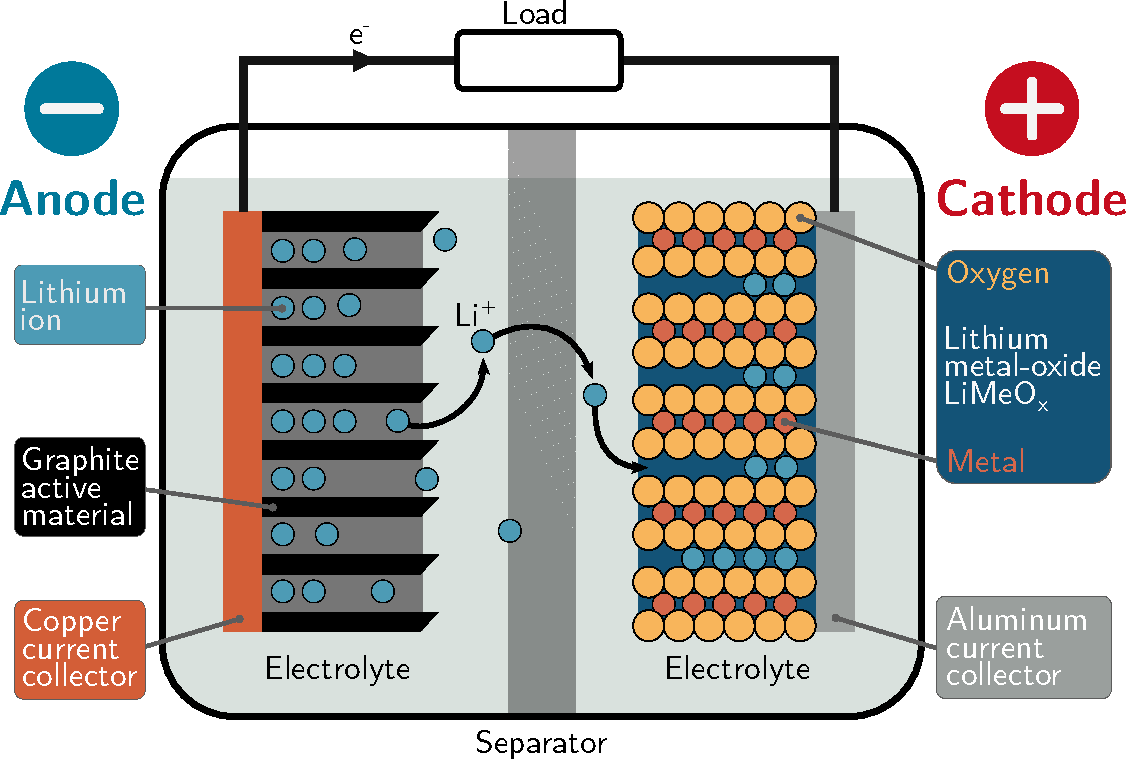
\includegraphics[width = \textwidth]{pictures/LIB.pdf}
\caption[Buildup LIB]{Schematic of a general \gls{lib}}
\label{libsc}
\end{figure}

In the \gls{lib} the lithium-ions are responsible for the storage of energy. During charging and discharging the ions are moved from the anode to the cathode and vice versa. It is not necessarily always the case in all electrochemical systems that the main ion is moved during the reaction. Even though there always has to be an ion moving inside of the cell to close the electrical circuit, e.g. in lead-acid batteries the moving ion is a hydrogen ion, not a lead ion. \par The \textbf{electrolyte} in \glspl{lib} is not taking part in the cell reaction as it was the case in its technological predecessors, the nickel-hydroxide and lead-acid batteries, but is solely in the cell for the ion transport. For this reason the amount of electrolyte in the cell can be reduced to a minimum necessary to properly connect all the cell elements. Normally the electrolyte of commercial \glspl{lib} is composed of an organic solvent with a lithium salt as the lithium-ion source. The usage of a aqueous electrolyte in cell cells containing lithium is not possible, since lithium reacts with water. Typically the electrolyte is composed of a mixture of organic solvents to get the best performance. The most common solvents used are a combination of \gls{ec} and \gls{dmc} with \gls{lipf6} as the lithium containing salt. This combination has proven to have a good combination of temperature stability, good ion conductivity, good wetting ability and not co-intercalation. In the first \glspl{lib} models \gls{pc} was used, a remainder of the short-lived \gls{lmb} period, having a even better lithium-ion conductivity. This however was causing quick anode degradation when the solvent molecules undesirably intercalated into the graphite together with the lithium ions \cite{K.Brandt.1994}. The electrolyte also plays a mayor role in the formation of the \gls{sei} layer, that impacts the cell performance as well as the cell degradation and will be explained in detail in chapter \ref{seilayer}. \par
The \textbf{separator} is an element in any electrochemical cell that is physically separating the the two electrodes whilst electrically isolating them against each other. At the same time the separator must be permeable for the ion current inside of the cell, which in most cases means a porous separator that is permeable for the electrolyte. In \glspl{lib} the most common separator is a polymer membrane, e.g. made of \gls{pp} or \gls{pe}. The desired properties of the separator are a low weight, high thermal and mechanical stability and low material costs \cite{Deng.2015}.

\subsubsection{Charging and Discharging}
In a fully charged \gls{lib} all lithium-ions are intercalated inside of the anode. Intercalation means that the ions are positioned in between the graphite layers, but no chemical reaction has taken place. It is described by a reversible process that is keeping the structural integrity of the intercalation host material \cite{Li.2019}. The fact that there is no chemical reactions  is one factor of the high lifetime of \glspl{lib}. Since there is no new compound forming, the stress due to rearrangement of the material during the charging and discharging process is very low. The graphite is increasing in size by less than 10\% during the lithium-ion intercalation \cite{Winter.1998}. When the battery is discharged the lithium-ions de-intercalate from the anode by releasing one electron becoming \ce{Li+} and move through the electroylte to the cathode, where they are reacting with the metall-oxide to form a lithium-metal oxide. The cell total cell reaction in the discharge direction can then be described as:

\begin{align*}
\ce{Li_xC6 + Li_{1-x}MeO_y <=> C6 + LiMeO2}
\end{align*}

Where the x describes the ratio of lithium remaining within the anode, this number is equivalent to the \gls{soc}. The graphite can have different lithiation-states that can be seen in plateaus in the \gls{ocv} \cite{Bauer.2016}. The \ce{Me} is representative for a group of metals that can be used in the cathode. \par
During the charging process, this reaction is simply inversed and the lithium-ions are moving from the cathode to the anode, where they are intercalating into the graphite and take in one electron. \par
Since \glspl{lib} are very sensitive to over- and undercharging, it is very important to stay within the voltage limits for the given material combination. For this reason the most common choice of charging method for \glspl{lib} is the \gls{cccv} charging method. Using this method, the cell is charged with a constant current until the end-of-charge voltage is reached (typically \SI{4.2}{\volt}) and then that voltage is held during a constant voltage phase while the current drops. When the current reaches a minimum current threshold, the charge is finished. The minimum current is necessary due to self discharge and parasitic currents, because of which the charging current can never reach zero in a real application. Figure \ref{cccv} shows the voltage, current and \gls{soc} curves for \gls{cccv} charging, where $I_{ch}$ is the charging current and $I_{thres}$ the threshold current at which the charging process is terminated. $V_{max}$ and $V_{min}$ denote the end-of-charge and end-of-discharge voltage window of the battery, respectively.

\begin{figure}[ht]
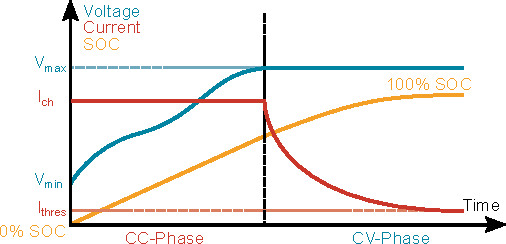
\includegraphics[width = \textwidth]{pictures/CCCV.pdf}
\caption[CCCV]{Voltage, Current and \gls{soc} curves of a typical \gls{cccv} charging process}
\label{cccv}
\end{figure}

During the CC-phase the majority of charge is put into the battery and the SOC is raising linearly. In most cases the battery is charged to around 80\% \gls{soc} in the CC-phase. The CV-phase then charges the remaining amount to 100\% \gls{soc}. The CC-phase makes up around half of the total charging time. For this reason a lot of fast-charging methods only use the CC-phase for charging and don`t use the full battery capacity.

\subsection{Anode}
Graphite is currently the most used anode material for lithium-ion batteries due to its high practical capacity and low potential vs \ce{Li}, enabling it to store a high amount of energy, and a rather flat discharge curving, giving a constant power output over a big range of the capacity \cite{Li.2019}. The anode of a commercial \gls{lib} as of today is in most cases made of a slurry of graphite (\ce{C6}) with added binder and carbon black that is pressed on a copper foil. The binder used is typically \gls{pvdf} \cite{Wang.2017}. The carbon black is added to increase the electric conductivity of the active material. The carbon has the shape of particles with varying sizes depending on the producer. Differently sized particles can have different effects on the cycle-lifetime and other parameters of the battery performance, like the available power density. \par
The anode is typically oversized compared to the cathode to prevent lithium plating at the edges \cite{Agubra.2013}. If the electrodes had the same size the increased electrical field strength at the edges of the anode could lead to lithium plating in these regions. This is sometimes also called the anode overhang.

\begin{figure}[ht]
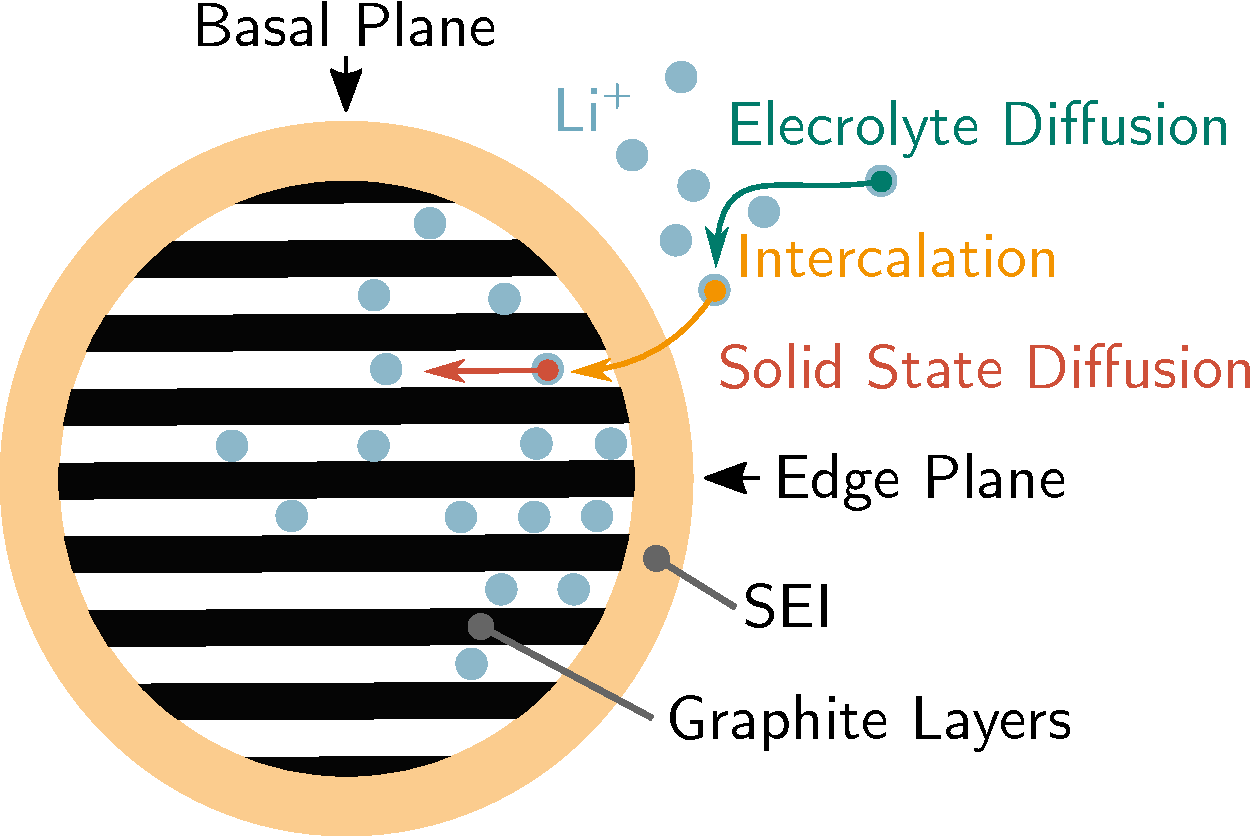
\includegraphics[width = \textwidth]{pictures/Anode_Particle.pdf}
\caption[Anode graphite particle]{Schematic view of one graphite particle inside the anode active material}
\label{graphiteParticle}
\end{figure}

All graphite particles also consist of basal and edge planes. The edge planes are perpendicular to layer direction of the graphite crystals. They provide an easy entry point for the lithium-ions to intercalate into the Graphite. This is why most of the lithium-ion insertion and diffusion into the active material starts from the edge planes. The basal planes are along the layer direction of the graphite crystal and lithium-ions cannot intercalate across a basal plane into the graphite, which is why they are the less reactive areas of the graphite particles. The ratio of edge planes to basal planes has a high impact on the electrochemical performance of a given graphite material \cite{An.2016}. The same way the orientation of the particles has a similar influence, with less oriented graphite generally having a worse performace due to a more difficult diffusion for the lithium ions \cite{Agubra.2013}.  \par
In the charged state the lithium-ions are intercalated into the graphite, located between the graphite planes. Lithium can naturally diffuse into graphite and is evenly distributing in the anode active material over time after the charging in finished. The resulting material of graphite with intercalated lithium-ions is called a \gls{gic} that is characterized by a mixed ionic and electric conduction \cite{Li.2019}. \par
The volume expansion of graphite (\ce{C6}) compared to fully lithiated graphite (\ce{LiC6}) is approximately at about 10\% to 13\% when the lithium-ions inhabit the free lattice spots within the graphite \cite{Lin.2016,Li.2019}. This effect is quite low compared to other materials, but still leads to mechanical stress inside of the cell during cycling. \par
To avoid lithium plating due to anode overcharging, explained in more detain later in chapter \ref{liplating}, the anode is usually oversized by around 10\% compared to the cathode \cite{Gallego.2014}.

\subsubsection{Anode Ageing}
In general ageing of all cell components can be divided into calendar ageing and cyclic ageing. Calendar ageing describes the chemical degradation over time due to unwanted mostly unavoidable side reactions. Cyclic ageing on the other hand describes the stress on the cell components during cycling, i.e. in case of a \gls{lib} when the lithium-ions are shifted from anode to cathode and vice versa. For calendar ageing the main influencing factors are the temperature and the \gls{soc} of the cell. The result of battery ageing is typically loss of usable capacity and an increase of the internal resistance, leading to a lower available power density \cite{Lin.2015}. Depending on the occuring ageing mechanisms, there can be primarily capacity loss, primarily an increase in internal resistance or both. \par 
For the anode the main ageing mechanism is the formation, growth and reformation of the \gls{sei} layer, that forms on the surface of the graphite particles. This layer consumes lithium ions, reducing the available lithium inventory and at the same time increase the cell impedance. A  more detailed description of the ageing mechanism can be found in chapter \ref{seilayer}, since this layer also has a big impact on the lithium plating effect \cite{Lin.2015}.\par
Another ageing effect is the mechanical stress the anode receives during charging and discharging due to the change in volume of the cell. While the volume change of around 10 to 13\% is rather small, prolonged cycling can lead to contact loss between the graphite particles, the active material and the current collector and to a change in porosity of the anode material \cite{Vetter.2005}. Other sources of mechanical stress can be the co-intercalation of solvent ions, that can cause graphite exfoliation and gas evolution during electrolyte decomposition \cite{Lin.2015}. These mechanical ageing effects can affect the capacity, due to loss of active material or contact loss with the active material, or internal resistance due to longer diffusion paths \cite{Vetter.2005}. Over time the pores of the anode material can also be clogged with solvent decomposition products, leading to a higher charge transfer resistance \cite{Agubra.2013}. \par
The strongest effect on the capacity loss has the lithium plating, explained in more detain in chapter \ref{liplating}. Here an unwanted deposition of metallic lithium on the anode surface can happen under specific conditions, including charging at low temperatures and high charge currents \cite{Vetter.2005}. \par
Overall the capacity fade even under the same conditions are not linear with time can change depending depeding on those conditions \cite{Barre.2013}. 





\subsubsection{The SEI Layer}
\label{seilayer}
The \gls{sei} layer does not only have a huge impact on the cell performance, it also is the main reason for cell ageing in \glspl{lib} \cite{Vetter.2005}. The \gls{sei} is a thin layer on the anode surface that is forming due to electrolyte decomposition. There is no electrochemically stable electrolyte for the operating voltage range of a \gls{lib}, so a decomposition in unavoidable. Due to the high reactability of water with lithium an aqueous electrolyte is no option in the current state \glspl{lib}. The working voltage window in the battery will either cause electrolyte decomposition at the anode or cathode at the respective voltage values of a fully charged of fully discharged cell \cite{Wang.2018, Lin.2016}. The stability window for most of the commonly used electrolyte parts (e.g. \gls{ec},\gls{dmc}) is from around \SI{0.8}{\volt}  to \SI{4.7}{\volt} vs \ce{Li/Li+} \cite{Goodenough.2010,Palacin.2018}. This window is further decreased by the cell temperature leading to electrolyte degradation also at the cathode for elevated temperatures \cite{Shikano.2007,Rahman.2007}. As most commercially available \glspl{lib} operate from around \SI{0.2}{\volt} vs \ce{Li/Li+} when fully charged to \SI{1.7}{\volt} vs \ce{Li/Li+} when fully discharged, the decomposition takes place on the anode side at high \gls{soc}. In the decomposition process not only the components of the electrolyte are consumed, but also the lithium-ions present in the electrolyte. This does reduce the total number of available lithium in the cell and in consequence the capacity of the cell. This implementation of lithium-ion however into the \gls{sei} does enable lithium-ions from the electrolyte to pass through it to reach the anode surface. Without the lithium-ions in the \gls{sei} the cell could not function since the lithium-ions from the electrolyte could not intercalate into the anode surface. The decomposition reaction can also take place at voltages inside of the stable window, but in this case it was shown that the reaction is reversible since the electrolyte molecules stay intact \cite{Seidl.2016}. \par
Since the \gls{sei} is electrically insulating, the growth of the layer should in theory stop after its initial formation. In a real cell however there is always a small current due to electron hopping leading to a slow but constant \gls{sei} growth over time. This growth is accelerated with higher temperatures. During cell cycling the \gls{sei} can also be damaged due to the swelling and contraction of the anode during the lithium intercalation and de-intercalation, facilitating a reformation of the \gls{sei} at newly exposed anode surface. There can also be co-intercalation of other electrolyte components and gas evolution during the decomposition process causing extra stress on the \gls{sei}, with the highly flammable gas additionally posing a safety risk \cite{Seidl.2016,Balagopal.2018}. Due to the fact that the decomposition of existing \gls{sei} is different from the reaction on the anode surface, the mechanisms changes with a higher coverage of the electrode surface \cite{Wang.2018}. The \gls{sei} is not only gradually reducing the capacity of the cell but also having a major impact on the self-discharge characteristics, achievable power density and safety of the cell \cite{An.2016}. \par
These effects lead to a number of desired parameters that can create a stable \gls{sei} that can lead to a long cell life. The \gls{sei} should be as thin as possible while at the same time being highly electrically insulating to prevent further decomposition. Even if the material composition of the layer is technically electrically insulating, it needs to be thick enough to block electron tunneling \cite{Lin.2016}. But it should also be permeable selectively for lithium-ions for a low cell internal resistance. The layer should also be chemically inert towards all other cell components at a wide range of potentials and temperatures to prevent dissolving of parts of the \gls{sei} back into the electrolyte. To compensate for the change in anode volume during cycling it should also have a good mechanical stability to prevent breaking and subsequent reformation \cite{An.2016, Wang.2018}. The fracturing of the \gls{sei} is even reported to have a bigger effect on the capacity fade than the cracking of the underlying graphite particles due to the fact that is has a higher tendency to fracture \cite{Deshpandezand.2017}. \par
To achieve these desired \gls{sei} attributes, the cells are normally charged under special conditions by the manufacturer during their first charging cycles. This process is called cell formation. Before the formation process a full coverage of the anode with the electrolyte has to be assured. This is done by the wetting process, which is typically a prolonged period of resting time (sometimes at elevated temperatures) following the electrolyte filling. During the first cycle of the formation 10\%-20\% of the whole cell capacity are typically consumed for the \gls{sei} generation \cite{Patil.2008,Lin.2016,Gallego.2014}. The factors that the manufacturer can directly control during the formation process are the applied current, the different cut-off voltage levels and the temperature. These all can have a strong influence on the parameters and stability of the formed \gls{sei}, creating different microstructural and chemical properties that can lead to a different long-term chemical and mechanical performance \cite{An.2016}. The current during the formation is typically kept at very low C-rates, ranging from C/5 to C/20 \cite{Wood.2015}. Most of the \gls{sei} is theorized to be formed at \SI{0.2}{\volt} to \SI{1}{\volt} vs \ce{Li/Li+} \cite{An.2016}. Other parameters that can be adjusted in cell design that also influence the \gls{sei} formation are the graphite type, graphite morphology, electrolyte composition and electrolyte additives, but also factors like particle size of the graphite, basal-to-edge-plane ratio, pore size, degree of crystallinity, \ce{Li+} diffusion rate and chemical composition of the surface (e.g. impurities) can affect the \gls{sei} composition \cite{An.2016,Seidl.2016,Bhattacharya.2012}. A commonly used additive is \gls{vc}, preventing exfoliation during lithium intercalation in the beginning of the \gls{sei} formation \cite{Aurbach.1998,Flandrois.1999,Tasaki.2006}. Using bigger particles can lead to a smaller capacity loss during \gls{sei} formation since the surface to volume ratio is lower in this case, but these particles are also more prone to exfoliation \cite{An.2016}. The whole wetting and formation process can take up to 0.5 to 2 weeks \cite{Wood.2015} and needs dedicated cycling capacities for each single cell, make it one the most important bottlenecks of cell production. \par
The resulting layer has a thickness in the range of nano meters, with reported values going from 3 to \SI{120}{\nano\meter} \cite{An.2016,Bhattacharya.2012,Shinagawa.2017,Seidl.2016}, but other publications also report widely varying thicknesses in the micrometer range \cite{Bhattacharya.2012,Balagopal.2018}. Since the intercalation reaction happens on the edge planes of the graphite particles, the potential on these planes is higher than on the basal planes. This leads to a thicker and differently composed \gls{sei} on the edge planes \cite{Seidl.2016}. The thickness of the \gls{sei} is also varying with the position of the electrode, with the \gls{sei} generally being thinner towards the center, and dependent on the type of aging, being thicker when it is caused by calendar ageing \cite{Mussa.2019}. All these factors lead to a differing lithium diffusion constant throughout the \gls{sei} in different locations \cite{Bhattacharya.2012}. The pressure on the layer also influences the electron tunneling ability, with more tunneling when the layer is under tension and less tunneling if the layer is under pressure \cite{Lin.2016}. \par  
The chemical composition of the \gls{sei} layer is also highly dependent on the conditions under which the layer is formed. A loose organic \gls{sei} with rather low conductivity for the lithium-ions is formed at higher charging anode potentials and more compact inorganic structures with higher ion conductivity at lower potentials \cite{Bhattacharya.2012,Tran.1996}. The charging rate on the first formation cycles on the other hand affects the porosity of the layer, with a more porous layer and higher resistance at higher charging rates. Water residue in the graphite can cause \ce{HF} creation in electrolytes with \ce{LiPF6}, which is the most commonly used salt in modern lithium ion batteries. The \ce{HF} can then attack the \gls{sei} and cause a drop in performance of the \gls{lib} \cite{An.2016}. The overall structure of the \gls{sei} can roughly be described as a multi-structure bilayer \cite{An.2016,Wang.2018,Bhattacharya.2012,Lin.2016}. The edge sites mainly contain a loose layer filled with electrolyte of inorganic lithium carbonates, organic lithium alkali carbonates and polymeric compounds on the side facing the electrolyte, while the graphite site is a more dense layer of \ce{LiF}, \ce{Li2O} and \ce{Li2CO3} \cite{Peled.1998, Eshkenazia.2004}. Between these two phase a mixed layer can be found. In general it can be said, that the \gls{sei} compounds closer to electrode are reduced stronger than the compounds in contact with the electrolyte \cite{Seidl.2016}.  On average more than half of the \gls{sei} is composed of \ce{LiF} and \ce{Li2Co3}. Compared to the edge sites, on the basal site a higher concentration of lithium carbonates can be found on the electrolyte site, and a lower content of \ce{LiF} \cite{Peled.1998,Eshkenazia.2004}. The whole composition is on the basal sites is also less organic \cite{Seidl.2016}. To prevent the loss of the \gls{sei} due to re-dissolution into the electrolyte \cite{Wang.2018}, it is desired to create a layer mainly composed of inorganic components like \ce{Li2CO3} rather then \ce{ROLi} or \ce{ROCO2Li}. The \ce{ROCO2Li} can react with traces of \ce{CO2} or \ce{H2O} present to form lithium carbonate \cite{Lu.2008}. Hao et al.\cite{Hao.2017} also notes, that the lithium ion concentration in the \gls{sei} highly fluctuates due to an heterogeneous \gls{sei} structure. The micro structure is also reported to contain nano-crystalline domains of 5-\SI{20}{\nano\meter} in size manly consisting of \ce{Li2CO3} and \ce{Li2CO2} \cite{Bhattacharya.2012}. In some cases elements from the cathode can cross over to the anode and cause \gls{sei} growth, as shown for \ce{Mn2+} ions \cite{Leung.2017}. \par
The analysis of the \gls{sei} is very hard due to its very small layer thickness and sensitivity to oxygen and moisture \cite{An.2016}. To get a deeper understanding of the \gls{sei} a number of different measurement and modeling approaches have been used, including ab initio molecular dynamics (AIMD) simulations \cite{Soto.2018}, to get insight into the reaction dynamics,  \cite{Shinagawa.2017} et al. using a monte carlo simulation to determine the relationship between the layer thickness and its lithium ion conductivity, a mathematical model proposed to describe the mechanical stress on the \gls{sei} and subsequent fracturing during cycling \cite{Deshpandezand.2017}, while \gls{afm} was used in \cite{Bhattacharya.2012} to measure the thickness and coverage of the \gls{sei}. \par
The continuous growth of the \gls{sei} layer over the lifetime of the cell depends on a lot of factors. Firstly a higher cell temperature increases the growth rate since in increases the reaction rate of all chemical reactions within the cell. High temperature can also lead to a change in the composition and morphology of existing \gls{sei} \cite{Palacin.2018}. Secondly mechanical stress can lead to the braking and subsequent reformation. This is dependent on the charging speeds and flexibility of the \gls{sei}. And lastly the aforementioned crossing over of cathode metals that can influence the chemical reactions within the \gls{sei}.\par
The \gls{sei} layer also has a profound impact of the plating behavior of cells. The thickness and ion conductivity of the layer directly influences the potential drop at the anode surface, which is the main driving force of the plating process. The mechanical properties of the layer can influence the morphology and shape of plating, i.e. whether the plated lithium metal forms as a homogeneous layer or in the form of located dendrites, that can cause potential risk to the cell safety \cite{Bieker.2015}.

\subsubsection{Lithium Diffusion}
The lithium diffusion inside of the graphite is one of the key drivers on lithium plating. Within the cell there are two different diffusion processes for the lithium-ions. One is the diffusion through the electrolyte, which is in a magnitude of 0.4 to \SI{1.4d-5}{\square\centi\metre\per\second} \cite{Lee.2002}. The second part of the diffusion is the solid state diffusion in the graphite particles occurring when then concentration of lithium ions is non-homogeneous within the anode. This happens whenever ions are removed from, or added to the anode, i.e. during charging and discharging, since the transfer of the ions from the electrolyte to the anode is faster than the distributing of the ions inside of the active material. The ions are capable of moving along the vertical direction between the graphite lattice layer since the bonding between the layers is comparably weak, leaving a gap of \SI{3.35}{\angstrom} in which the ions can move and intercalate \cite{Li.2019}. Since the magnitude of the solid state diffusion is much lower that the value for the electrolyte \cite{Kulova.2006} the diffusion inside of the graphite is one of limiting factors to reach high charging speeds and also the key factor for the occurrence of lithium plating. The value of the  diffusion for the solid state phase varies strongly from publication to publication, spanning everything from \SI{10d-16}{} to \SI{10d-6}{\square\centi\metre\per\second} \cite{Kulova.2006,Persson.2010}. The main cause of this big difference stems from the fact that the diffusion rate is dependent on multiple different parameters. \par
Firstly, the diffusion is dependent on the temperature , with lower diffusion rate at lower temperatures, that can be described by the Arrhenius equation \cite{Kulova.2006}. The diffusion of lithium ions starts at a temperature of \SI{230}{\kelvin} \cite{Umegaki.2017}. Secondly, it is also dependent on the \gls{soc} of the anode,i.e. the amount of lithium that is already intercalated into the  \cite{Malifarge.2018}, although this is effect is described to be of lower influence than the effect of the temperature \cite{Yu.1999,Levi.1996}. This make sense as with a higher intercalation depth, the mobility of the lithium-ions is hindered by lithium-lithium interactions \cite{Persson.2010}. Furthermore the distribution of the lithium-ions inside the graphite is not smooth but rather in fixed intercalation levels, called stages. These stages change abruptly when the lithium concentration reaches a certain threshold and are visible in the charge and discharge curves in form of flat plateaus. The intercalation levels are the following \cite{Nowak.2014}:

\begin{align}
    \ce{LiC72 <-> LiC36 <-> LiC27 <-> LiC18 <-> LiC12 <-> LiC6} 
\end{align}



The evolution of these stage structures also influences the diffusion coefficient \cite{Li.2019}. Another point is that the diffusion along the edge planes is much higher than along the basal planes \cite{Persson.2010}. Thus the edge to basal rate, particle size and particle orientation of the graphite have a big impact on the diffusion rate as well. This is also true for defects and along the grain boundaries. Here the diffusion is also servery hindered \cite{Persson.2010}. Lastly, these parameters are also interconnected, with Umegaki et. al \cite{Umegaki.2017} showing that the temperature dependency is different for different intercalation stages. \par
All these influencing factors show that the diffusion coefficient can be vastly different even within the same cell, when particle orientation, size, local temperature, local defects, can differ. Thus the lithium plating process, directly affected by the diffusion coefficient, is highly localized on the anode surface and requires a spatially resolved analysis for deeper understanding.

\subsection{Cathode}
 The most commonly used metals used in the cathode are nickel, manganese and cobalt. Since all of these metals have different beneficial effects on the cell performance, a mixture of them can create a good compromise that can the best aspects of all the possible metals. Thus most cells today use a $\ce{Li(Co_{\frac{1}{3}}Ni_{\frac{1}{3}}Mn_{\frac{1}{3}})O2}$ mixture, where the fractions of the used materials can vary. These cells are called \gls{nmc}-cells. Research is aiming at reducing the amount of cobalt in the cells, since it is not only the most expensive of the used materials in the cell, it is also mined under questionable conditions for the workers as well as the environment \cite{Zubi.2018}. Apart from these metals there are also lithium-iron phosphate cells that are cheaper, have a long lifetime and comparably low environmental impact \cite{Deng.2015}, but the downside of a lower energy density, making them less suitable for mobile applications.\par
 Because of the fact, that the anode is oversized compared to the cathode, the cathode is never fully charged again after the initial cycle \cite{Palacin.2018}.
 
 \subsubsection{Cathode Ageing}
While the cathode of a \gls{lib} also plays a major role for the performance of the cell, the effect of the cathode on cell ageing and especially lithium plating is low compared to the anode. Lithium plating does happen on the cathode side since the potential of the cathode is very far away from the potential of metallic lithium. One noteworthy ageing mechanism, that also affects the \gls{sei} growth on the anode side of cell and thus can have an impact on lithium plating is the transition metal dissolution and migration \cite{Palacin.2018,Lin.2015,Agubra.2013,Vetter.2005}. Here the metal ions of the cathode can be dissolved into the electrolyte and then move over to the anode surface, where they can take part in the chemical processes at the \gls{sei} and change the structure, morphology and growth rate of the \gls{sei}, often leading to a higher capacity loss and self discharge. This effect is most pronounced with cathodes containing manganese and has a considerably lower impact with cobalt-nickle mixeoxides \cite{Amatucci.1996,Liu.2003}. On the cathode surface an \gls{sei} similar to the anode \gls{sei} can form at end of charge \cite{Palacin.2018}. The impact on the cell performance of the cathode layer however is much lower on the cell performance. This layers however can be isolating and thus lead an in-homogeneous current distribution in the cathode \cite{Agubra.2013}. \par
The cathode is also similarly to the anode subject to mechanical stress during the insertion of lithium ions, which can cause crystal distortion \cite{Lin.2015}. 


\begin{align*}
    A = b\cdot V_t
\end{align*}


\subsection{The Lithium Plating Process}
\label{liplating}

\subsection{The Lithium Plating Detection}
\subsubsection{XPS}
The high energy of an XPS beam spot could alter the chemical composition of the \gls{sei} \cite{Bhattacharya.2012}.